% xform-buffer.tex

\documentclass[tikz]{standalone}
\usetikzlibrary{shapes, positioning, arrows.meta, calc, intersections, backgrounds, fit}

% default horizontal/vertical distance
\def\hdist{2.2}
\def\vdist{0.8}
\tikzset{node distance = \vdist and \hdist}

\newcommand{\state}[3]{% #1: name; #2: position; #3: label
  \node (#1) [inner sep = 1pt, minimum size = 5mm, align = center, draw, #2, font = \scriptsize] {#3};
}

\newcommand{\trans}[5]{% #1: start state; #2: end state; #3: label position; #4: label; #5: style
  \draw[-, #5] (#1) to node [rectangle, draw, #3 = 2pt, sloped, inner sep = 2pt, font = \tiny] (#1#2) {#4} (#2);
}

\begin{document}
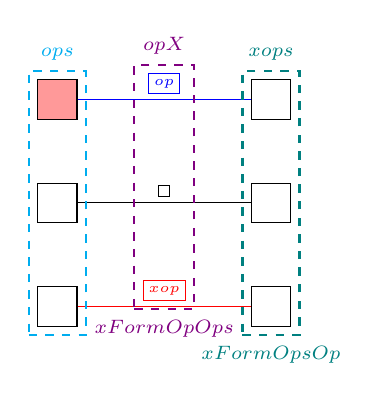
\begin{tikzpicture}
  \state{ops1}{fill = red!40}{}
  \state{ops2}{below = of ops1}{}
  \state{xops1}{right = of ops1}{}
  \state{xops2}{right = of ops2}{}

  \trans{ops1}{xops1}{above}{$op$}{blue}
  \trans{ops2}{xops2}{above}{}{}

  \state{ops3}{below = of ops2}{}
  \state{xops3}{right = of ops3}{}
  \trans{ops3}{xops3}{above}{$xop$}{red}

  \node (ops) [thick, dashed, cyan, font = \scriptsize, draw, inner sep = 3pt, fit = (ops1) (ops3), rectangle, 
  	label = {above: \textcolor{cyan}{\scriptsize $ops$}}] {};
  \node (opX) [thick, dashed, violet, font = \scriptsize, draw, inner sep = 3pt, fit = (ops1xops1) (ops3xops3), rectangle, 
  	label = {above: \textcolor{violet}{\scriptsize $opX$}},
  	label = {below: \textcolor{violet}{\scriptsize $xFormOpOps$}}] 
	{};
  \node (xops) [thick, dashed, teal, font = \scriptsize, draw, inner sep = 3pt, fit = (xops1) (xops3), rectangle, 
  	label = {above: \textcolor{teal}{\scriptsize $xops$}},
  	label = {below: \textcolor{teal}{\scriptsize $xFormOpsOp$}}] 
	{};
\end{tikzpicture}
\end{document}
